\chapter{Workload Metrics} \label{ch:workload}

The paper presented in chapter 2 was written before the workload concepts and modeling language semantics had settled into their current form.  Additionally, Jared et al., in concert with this work, published a paper in the FVHMS proceedings that expands on the concepts in chapter 2 but is also slightly outdated.  Thus we feel it expedient to summarize those aspects of the language which are critical to our metrics before we present the metrics themselves.  To assist in this effort we have prepared a simple scenario which includes a partial model and illustrations of the DiRG, DiTG, and labeled state transition system.

\section{Summary of workload concepts}
Show the labeled state transition system and talk about how it represents the scenario.

\subsection{Example Scenario}

In this scenario there are two main actors, Alice and Bob.  Alice is standing next to Bob listening to a friend on her cell phone.  Bob suddenly remembers that he wants to ask Alice out.  Not noticing that Alice is listening to her phone Bob starts to ask Alice on a date.  After listening to both her phone and Bob for a minute Alice looks at Bob and points to her phone.  Bob stops talking and decides between waiting for her to finish or walking away.  Eventually Bob walks away.

From the scenario above we chose to create two Actors, Alice and Bob.  Actors represent any aspect of the system that has state.  While in this scenario both our Actors are human, an Actor can be anything.  For example we could add lighting to the scenario and give it a light and a dark state.  We could also create a sub-Actor which is part of a larger Actor, such as Bob's hair, and give it states like messy or combed.  Actors can also be very abstract or very detailed.  The more states an Actor contains, the more expressive it becomes.

\begin{figure}[h]
\begin{center}
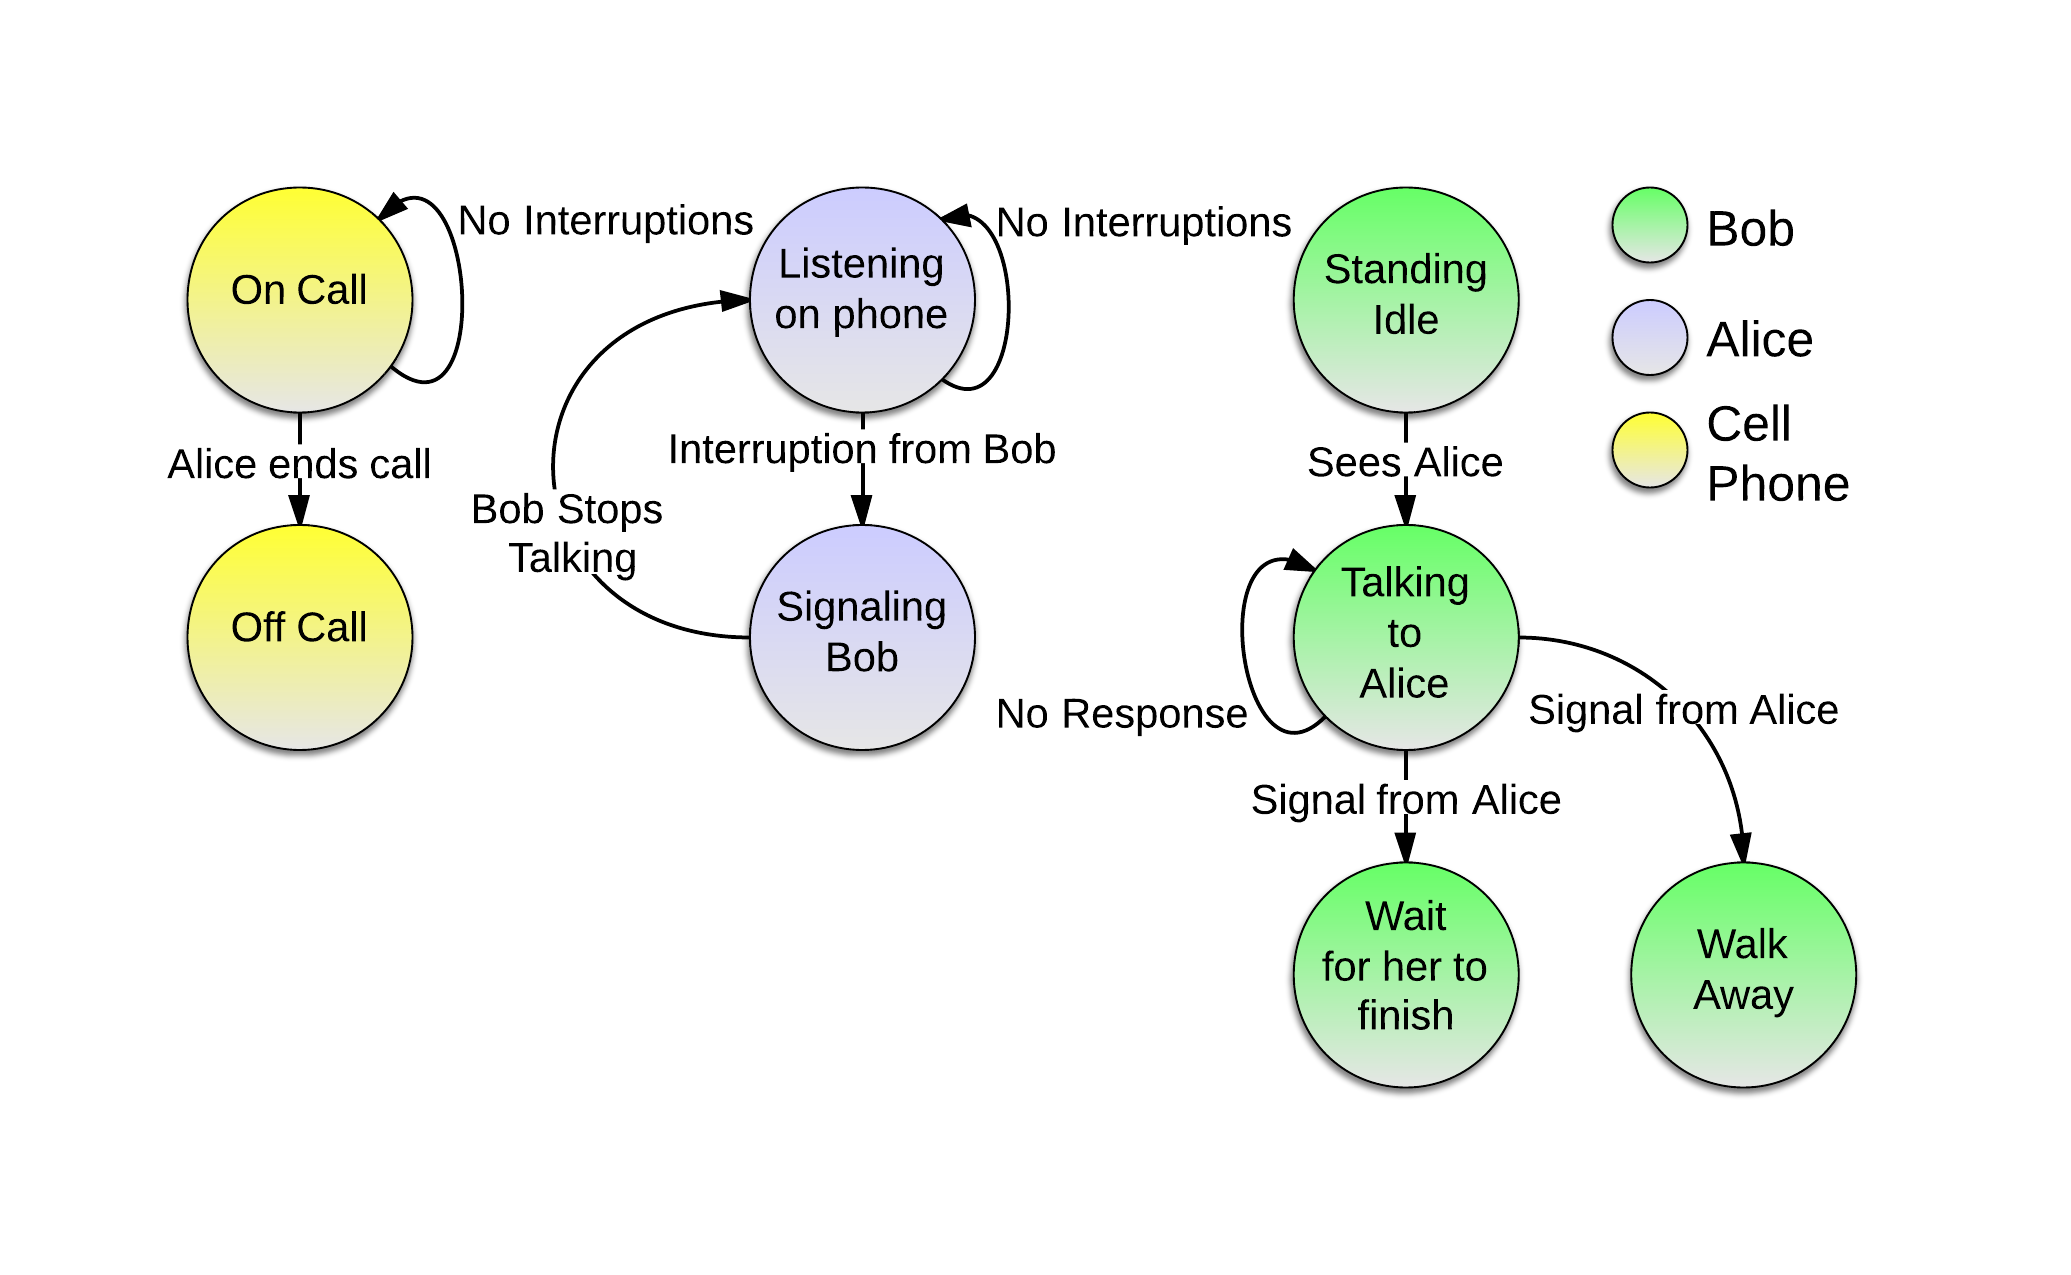
\includegraphics[width=\textwidth]{ab_dirg.png}
\caption{Directed Role Graph for Alice and Bob scenario}
\label{fig:ab_dirg}
\end{center}
\end{figure}

We express an Actor as a Directed Role Graph (DiRG).  A DiRG represents how an Actor is allowed to flow between states.  Figure~\ref{fig:ab_dirg} shows the DiRGs for both Alice and Bob as finite state machines.  We see that Alice is initially in a {\em Listening on phone} state while Bob is in the {\em Standing idle} state.  Alice can either stay in the {\em Listening on phone} state, shown by the looping transition, or move into the {\em Signaling Bob} state.  Once in the {\em Signaling Bob} state her only choice is to stay there forever or to return to the {\em Listening on phone} state.  Individually these DiRGs are of little value, together they begin to express the larger system.  We see from the labels on the DiRG that Alice and Bob are interacting with one another and influencing the transitions of the other.  Before we discuss Actor transitions we must first define how Actors can influence one another.

We define the connection between two Actors as a Channel.  A channel is a uni-directional communication medium which allows an Actor to send information to another Actor.  Each Channel is composed of a source Actor, a target Actor, and a type.  The source Actor sends information as {\em output}, the target Actor receives the information as {\em input}, and the type specifies which communication medium is being used.  In the case of Alice and Bob we use Audio and Visual Channels\cite{wickens2002multiple}, the case study in chapter \ref{ch:UASinNAS} also uses a Data channel that represents network communication.  While other researchers allow multiple channels of the same type to exist between Actors\cite{FVHMS}, for the scope of this paper we explicitly check that each Channel is unique.  


The Directed Team Graph (DiTG) 


In this and many other cases a single Actor is of little interest.  What is of more interest is a group of Actors working together.  This is expressed as a Directed Role Graph

For this scenario the first step to building our model is to define our Directed Role Graph (DiRG) and our Directed Team Graph (DiTG).  The DiRG is a collection of finite state machines.



\subsection{Labeled State Transition System}


\subsection{Directed Role Graph}
What is a Directed Role Graph.  Show the DiRG for Alice and Bob.
\subsubsection{Actors}
What is an Actor?  What does it represent?  Actor State?  Set of transitions for each state.  

\subsubsection{Events}
What are events? how are they used? intuition?

\subsubsection{Actor Load}
What is it? Intuition behind it?  How is it represented? Memory

\subsubsection{Transitions}
What is a transition?  What is an Active transition? Durations.  Input and Output.

\subsection{Directed Team Graph}
What is a DiTG.  What are the rules behind it.  Show the DiTG for Alice and Bob.

\subsubsection{Channels}
What is a channel?  Properties of a channel?  Intuition of a channel?  Layers of a channel?  Active vs Inactive.  Input vs Output

\subsubsection{Simulator}
Delta clock?  Get next transition.  Then fire the transition.

\section{Resource Workload}
Describe what it is, point reader towards FVHMS paper.  Present the metric itself with the equation.
Intuition behind it?

\section{Decision Workload}
Describe what decision workload is, point reader towards FVHMS paper.  Present the metric itself with the equation.
Intuition behind it?

\section{Adapted Wickens' Metric}
Reason for creating it, intuition.  What it is (copy paste).